\indent

We propose to study di-muon electroproduction on hydrogen using the CLAS12 detector in experimental Hall-B and the 11 GeV longitudinally polarized electron beam. The reaction - 
\begin{eqnarray}
ep\to e^\prime ~\mu^+ ~\mu^- ~p^\prime
\end{eqnarray}
will be studied in wide range of W, Q$^2$, t, and M$_{\mu\mu}$ (Q$^{\prime 2}$).  
Only the electron and the muon pair in the final state will be detected, the recoil proton will be reconstructed in the missing momentum analysis. For detection and identification of the $e\mu^+\mu^-$ final state the CLAS12 Forward Detector (FD) will be used after some modifications.
For this measurements, the CLAS12 Central detector will not be needed since as it will be shown in Section \ref{acc_simulations} there are no final state particles in the region kinematics of proposed measurements that will be produced in its detection region. But we still intend to use the solenoid magnet for protection of the forward detectors from M\"{o}ller electrons.


\subsection{Detector Configuration}
\indent

\label{detector}
The proposed experiment requires (a) detection of muons and (b) much higher luminosity than CLAS12 design luminosity. The luminosity limit for CLAS12 is mostly defined by the electromagnetic background, in particular from M\"{o}ller electrons flooding the forward drift chambers (FDC). In the nominal configuration, combination of the solenoid field ($\sim$ few Tesla) and the M\"{o}ller cone, a tungsten cone with an opening for the beam that covers region of angles up to $3$ degrees, ensure the acceptable occupancy in FDC at luminosity of $\sim 10^{35}$ cm$^{-2}$ sec$^{-1}$. This proposal aims to run with $\sim 50 ~-~ 100$ times higher luminosity. The detector configuration presented here is designed to provide high luminosity running capability and the detection of muons in the CLAS12 Forward Detector. 

The plane view of the CLAS12 (cut in (YZ) plane) is shown in Fig. \ref{fig:clas12}. As a simple solution, we propose to remove the High Threshold Cherenkov Counter (HTCC) and increase the size of the M\"{o}ller cone (shown in gold) to cover the whole acceptance region of HTCC (shown with red ellipse). In this case the forward drift chambers will be fully protected from any background generated in the target and will be able to handle higher luminosities. With adequate thickness this shielding will be used as absorber for charged hadrons in the muon detector, which is CLAS12 FD. For the detection of the scattered electrons, a compact, highly segmented PbWO$_4$ calorimeter will also be used, which will be part of the shielding.  

\begin{figure}[h]
\centering
%\begin{picture}(80,60)
%\put(-120,-100)
{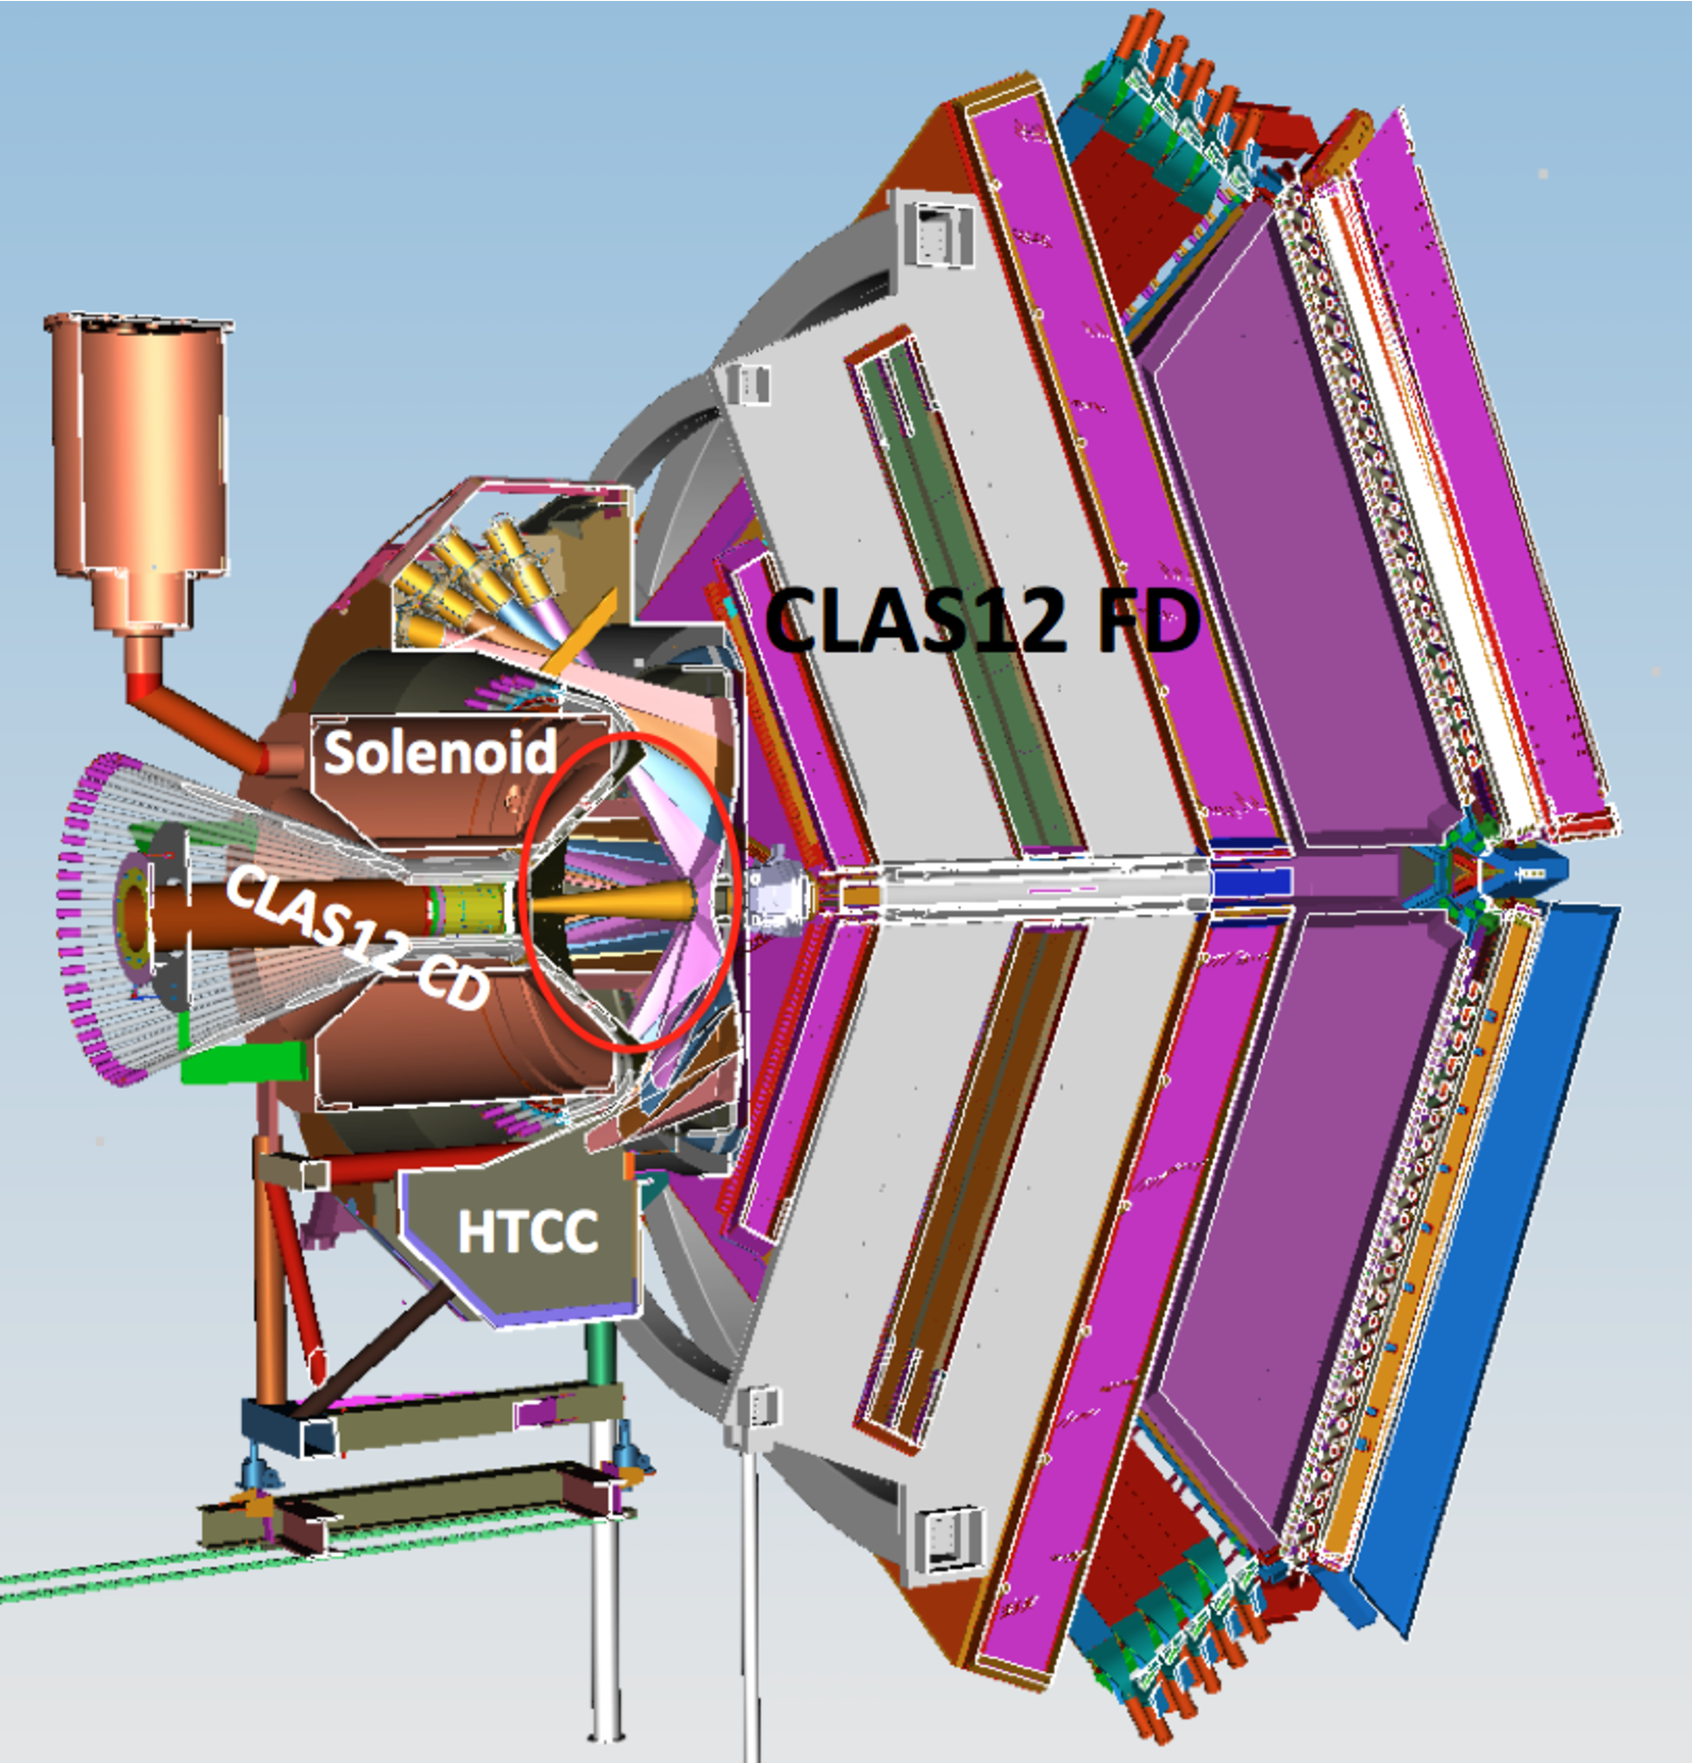
\includegraphics[width=0.9\textwidth]{clas12.pdf}}
%\put(-5,150){Solenoid}
%\end{picture}
\caption{The CLAS12 detector in Hall-B, mid plane cut view. The region of the working volume of HTCC is shown with red contour.}
\label{fig:clas12}
%\end{center}
\end{figure}

A concept of such shielding-calorimeter is shown in Fig. \ref{fig:shield}. The shield is $60$ cm thick and starts at $100$ cm from the target center. It extends to $35$ degrees in polar angle, the full range of the CLAS12 FD. The calorimeter used for the detection of the scattered electrons covers a polar angular range from $5$ to $35$ degree, and has $\pi/3$ in azimuthal coverage. The coverage and granularity of the calorimeter will be optimized with further simulations. 

\begin{figure}[h]
\begin{center}
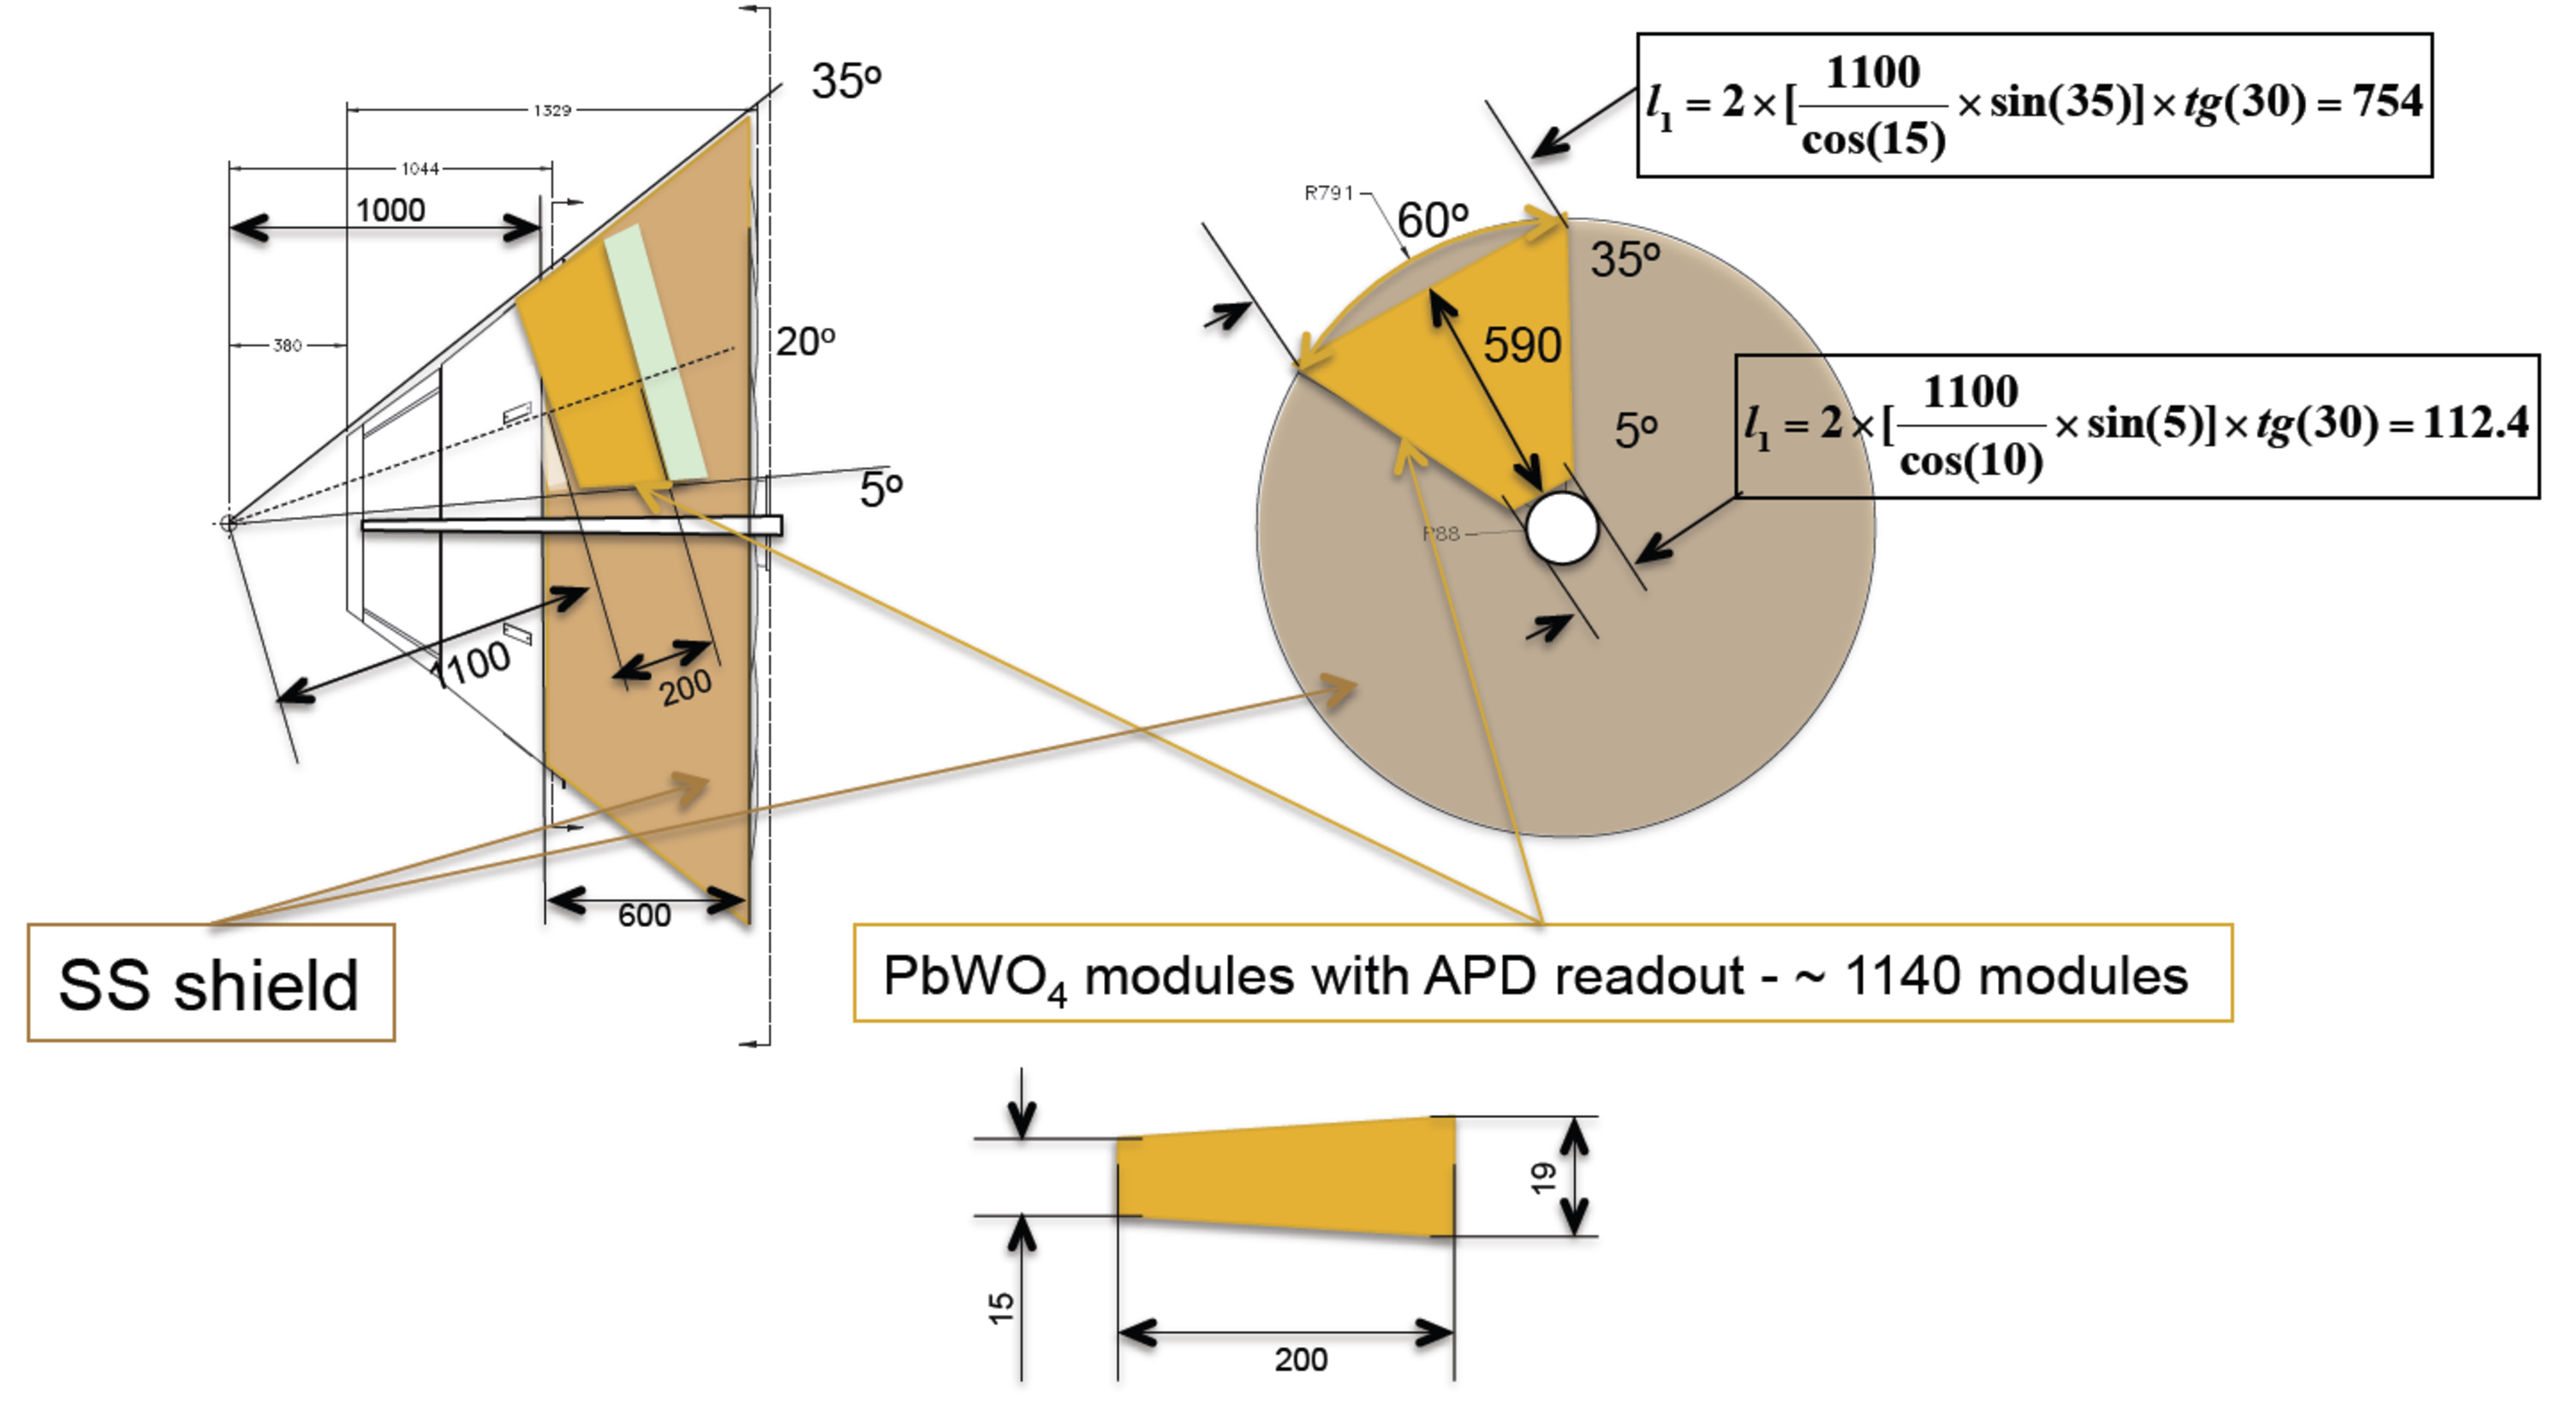
\includegraphics[width=1.\textwidth]{detector_concept.pdf}
\caption{The concept of the proposed shield and PbWO$_2$ calorimeter in the place of HTCC working gas. Dimensions on the figure are in mm, the size of PbWO$_4$ crystals are not optimized.}
\label{fig:shield}
\end{center}
\end{figure}


\clearpage